% !TEX encoding = UTF-8 Unicode
\documentclass[a4paper,11pt]{book}
\usepackage[utf8x]{inputenc}
\usepackage{fancyhdr}
\usepackage{a4wide}
\usepackage{ulem}
\usepackage{epstopdf}
\usepackage[frenchb]{babel}
\usepackage[T1]{fontenc}
\usepackage{amsmath,amssymb,amsthm,bbm} % math, mathbb, mathbbm
\usepackage{makeidx} %% index
\usepackage{rotating} %% pour rotate
\usepackage{multirow} %% pour regrouper un texte sur plusieurs lignes dans une 
\usepackage{color}
\usepackage{listings}
\usepackage{tikz,pgfplots,pgf}
\usetikzlibrary{arrows,shapes,arrows,positioning,calc,trees,snakes,plotmarks}
\usepackage{caption}
\usepackage{subfigure}
\usepackage{hyperref}
\usepackage{array}
\usepackage[final]{pdfpages} 
\usepackage{tikz}
\usepackage{titlesec}
%\usepackage{fourier}

% nouveaux environements de theoreme
%----------------------

\newenvironment{warning} 
   {~\\ \textbf{Attention !}}{\\} 


\theoremstyle{definition}
\newtheorem{proposition}{Proposition}
\newtheorem*{instruction}{Instruction}
\newtheorem*{fonction}{Fonction}
\newtheorem*{operation}{Opération}
\newtheorem*{declaration}{Déclaration}
\newtheorem{lemme}{Lemme}
\newtheorem{theoreme}{Théorème}
\newtheorem*{definition}{Définition}
\newtheorem*{syntaxe}{Syntaxe}
\newtheorem*{org}{Organigramme}
\newtheorem{exemple}{Exemple}[section]

\renewcommand*\thelstnumber{\arabic{lstnumber}:}
\renewcommand\lstlistingname{Programme}
\renewcommand\lstlistlistingname{Liste des programmes}

%----------------------------------------------------------------------------------------------------
% DEFINITION DU TITRE, DE L'AUTEUR ET DE LA DATE DU DOCUMENT
%----------------------------------------------------------------------------------------------------
\title{M105: Programmation}	
\author{Vincent Choqueuse }	
\newcommand{\annee}{2015}
\date{Septembre 2015}													
\addto\captionsfrench{\def\figurename{{Figure}}}
\addto\captionsfrench{\def\tablename{{Tableau}}}

%---------------------------------------------------------------------------
% PARAMETRAGE DES HYPERLIENS
%----------------------------------------------------------------------------------------------------
\hypersetup{
	colorlinks=true,	% Colorise les liens
    	breaklinks=true,	% Permet les retours à la ligne pour les liens trop longs
    	urlcolor= blue,		% Couleur des hyperliens
    	linkcolor= black,	
    	citecolor= green	% Couleur des liens vers les références bibliographiques
}



\definecolor{vert}{rgb}{0.2,0.6,0.4} 
\definecolor{rouge}{rgb}{0.9,0.,0.} 
\definecolor{iutbleu}{RGB}{46,88,134}

\makeindex


\pagestyle{fancy}
\rhead{}
\chead{}
\lhead{\slshape \leftmark }
\lfoot{IUT GEII Brest}
\rfoot{Automne \annee}
\cfoot{\thepage}
\renewcommand{\headrulewidth}{0.4pt}
\renewcommand{\footrulewidth}{0.4pt}
\setlength{\headheight}{20pt} 


\begin{document}
\thispagestyle{empty}
\lstset{language=C,showstringspaces=false,basicstyle=\ttfamily,stringstyle=\small,numbers=left,numberstyle=\footnotesize,frame=single,commentstyle=\upshape,framexleftmargin=7mm,xleftmargin=8mm,morekeywords={operation},captionpos=b}
\thispagestyle{empty}
\includepdf[pagecommand={\begin{tikzpicture}[remember picture, overlay]
\node[color=black,yshift=28.5em,xshift=-8.5em] at (current page.center) {\fontfamily{qag}\selectfont \Huge M105: Programmation};
\node[color=iutbleu,yshift=-5em] at (current page.center) {\fontfamily{qag}\selectfont \Huge \textbf{Cours}};
\node[color=iutbleu,yshift=-26em] at (current page.center) {\fontfamily{qag}\selectfont \large \textbf{Enseignants:} Vincent Choqueuse };
\node[color=iutbleu,yshift=-28em] at (current page.center) {\fontfamily{qag}\selectfont \large \textbf{contact:} vincent.choqueuse@univ-brest.fr};
\node[color=white,yshift=13.5em,xshift=5.7em,rotate=90] at (current page.center) {\fontfamily{qag}\selectfont \Huge \textbf{\annee}};
\end{tikzpicture}}]{./theme/cover_iut.pdf}

\thispagestyle{empty}

\tableofcontents

\newpage
\listoffigures
\newpage
\newpage
\lstlistoflistings
\newpage



\title{Cours de langage C}

\chapter*{Introduction}
\addcontentsline{toc}{chapter}{Introduction}

\section*{\`A qui s'adresse ce cours ?}

Ce cours s'adresse à des débutants en programmation. Le background nécessaire pour l'appréhender se limite à des bases de mathématique et d'informatique.

\section*{Déroulement de l'enseignement}
Ce cours est une initiation au langage de programmation C. Le langage C est avant tout un langage. Tout comme l'anglais, l'arabe, les hiéroglyphes, le langage C possède son propre vocabulaire et sa propre syntaxe. Contrairement aux langages précédents qui permettent aux hommes de communiquer entre eux, le langage C permet à l'homme de communiquer avec la machine (l'ordinateur, les smartphones, ...). \\

L'enseignement est composé de 20H de Cours-TD-TP. L'acquisition des connaissances sera évaluée au moyen de:
\begin{itemize}
\item Deux devoirs sur table.
\item Quatres devoirs de Travaux Pratiques sous Code::Block.
\end{itemize}

\section*{Pour en savoir plus}

\begin{itemize}
\item OpenClassrooms \cite{ZER}: Ce site propose des cours d'une excellente
qualité pédagogique. Après chaque leçon, il est possible de
tester ses connaissances en effectuant des quizz notés.
\item C Programming Language \cite{KERN88}: Livre de référence en anglais sur la programmation en C écrit par les développeurs du langage.
\end{itemize}

\chapter{Débuter en programmation}

En l'espace d'une 20aine d'année, le champs d'application des technologies numériques s'est développé très rapidement. Par rapport à l'analogique, la technologie numérique possède de
nombreux avantages (prix, facilité de copie de l'information, ...) qui ont permis son ascension rapide. 

Le langage binaire (suite de 0 et de 1) est la base de la
technologie numérique. Malgré sa simplicité apparente, ce langage
est difficilement compréhensible par l'homme sous sa forme initiale.
Pour dialoguer plus facilement avec les machines, les
informaticiens ont mis en place des langages de programmation. Ces
langages sont situés à mi-chemin entre le langage de la machine et le langage de l'homme supposé anglophone
\footnote{Pas de soucis ici si l'anglais n'est pas votre "cup of
tea" ! Les langages de programmation ne comportent qu'une minuscule
partie du dictionnaire anglais}. Chacun
pouvant créer son propre langage, de nombreux langages de
programmation ont vu le jour~\cite{HIST}. L'ensemble
de ces langages peut se diviser en plusieurs catégories suivant le paradigme de programmation utilisé: 
\begin{itemize}
\item les langages impératifs: C, Pascal, Fortran, Python
\item les langages orientés objets: Java, C++, C\#, Objective C, Python, Smalltalk
\item  les langages logiques: Prolog, ...
\item ...
\end{itemize}
Le choix d'un langage particulier dépend de l'application visée.
Dans le contexte des jeux vidéos, les langages C et C++ sont des
références incontournables. Concernant les applications pour
téléphones portables, l'Iphone d'Apple utilise un langage orienté objet dérivé du C (l'Objective C) alors que les téléphones sous Android utilise le langage orienté objet Java. Quant à lui, le monde d'internet est le berceau du PHP ou du Python du côté serveur, et du combo HTML5/ CSS3/  Javascript du côté client. Quel que soit le langage utilisé, tous reposent sur une méthodologie et une rigueur qu'il vous faudra acquérir pour être capable de vous adapter à n'importe quelle situation.

Dans ce cours d'initiation à la programmation, nous allons nous
intéresser à un langage impératif: le langage C. Ce choix est
motivé par plusieurs raisons. D'une part, les langages impératifs sont
souvent plus simples à appréhender et de ce fait représentent un
point de départ incontournable pour débuter en programmation.
D'autre part, parmi les langages impératifs, le langage C reste
un des langages les plus utilisés au monde malgré son âge (voir table \ref{pop_langage}). En
effet, le C possède l'avantage d'être rapide, portable et d'être à
la base d'autres langages plus évolués comme le C++, le C\# et l'Objective C.


\begin{table}[!h]
\centering
\begin{tabular}{p{2.5cm}p{3cm}p{3cm}r}
  \hline
  % after \\: \hline or \cline{col1-col2} \cline{col3-col4} ...
  \textbf{Position} & Langage & Type & Utilisation \\
  \hline
 \textbf{1}  & Java &Objet & $19.565\%$\\
 \textbf{2} & C & Impératif&$15.621\%$\\
 \textbf{3} & C++ & Objet&$6.782\%$\\
 \textbf{4} & C\# & Objet&$4.909\%$\\
 \textbf{5} & Python & Impératif-Objet&$3.664\%$\\
 \hline
\end{tabular}
\caption{Popularité des langages de programmation (indicateur Septembre 2015 \cite{TIO}) }
\label{pop_langage}
\end{table}

\section{Environnement de développement}

Pour réaliser un programme, il est nécessaire d'utiliser un
environnement de développement. L'environnement de développement
permet d'écrire des listes d'instructions, d'identifier
d'éventuelles erreurs de programmation, de transcrire le programme
en binaire, etc. Il existe différents environnements de
développement permettant de programmer en langage C. Dans ce
cours, nous allons utiliser Code::Blocks~\cite{COD}. Cet
environnement possède l'avantage d'être gratuit et relativement complet.
L'installation de Code::Blocks s'obtient en suivant les étapes
suivantes:
\begin{enumerate}
\item Aller à l'adresse suivante: \url{www.codeblocks.org/}.
\item Aller dans le menu vertical \texttt{Download}, puis aller dans la section \texttt{Download the binary release}.
\item Télécharger la dernière version de Code::Blocks.
\item Lancer l'installation de Code::Blocks.
\end{enumerate}

\begin{warning}
Assurez-vous de bien installer la version intégrant le compilateur GCC (fichier \texttt{codeblocks-13.12mingw-setup.exe}).
\end{warning}

\section{Mon premier programme}\label{corps}

Dans cette section nous allons créer notre premier programme en langage C sous Code::Blocks. Ce premier programme permettra de vérifier que l'installation de l'environnement s'est réalisée correctement. Les étapes suivantes décrivent la marche à suivre:
\begin{enumerate}
\item Lancer Code::Blocks
\item Aller dans \texttt{create a new project}.
\item Choisir \texttt{console application} pour créer un projet en mode console.
\item Appuyer sur \texttt{next}, choisir le langage \texttt{C}, puis appuyer sur \texttt{next}.
\item Donner le titre \texttt{mon\_premier\_programme} à votre projet, puis appuyer sur \texttt{next}.
\item Appuyer sur \texttt{finish}.
\end{enumerate}
Lorsque le projet est créé, Code::Block stocke le code source du programme dans le fichier \texttt{main.c}. Pour y accéder rapidement, il suffit d'ouvrir le contenu du dossier \texttt{sources} situé à gauche de l'écran. Si tout se passe correctement, l'écran affiche une fenêtre similaire à celle de la figure \ref{figcode}. Le contenu du fichier \texttt{main.c} est présenté dans le programme \ref{firstprog}.
\begin{figure}
\centering
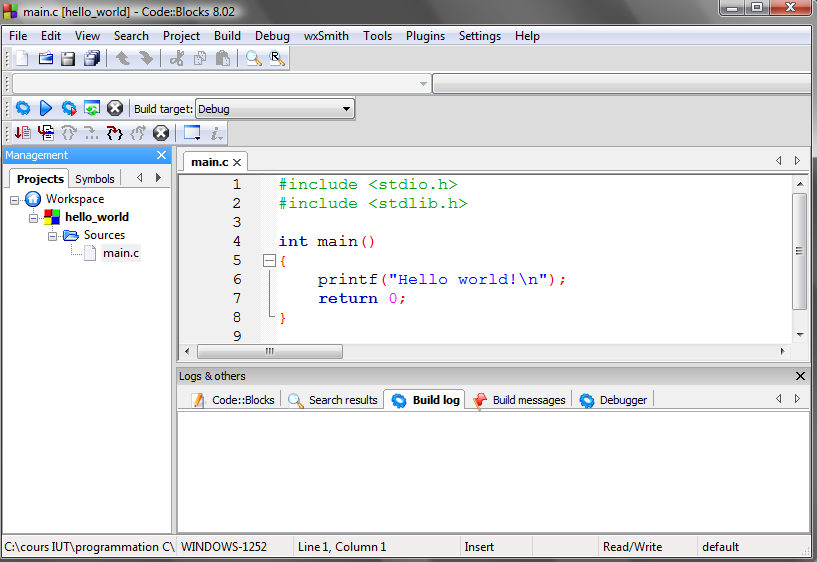
\includegraphics[width=0.9\linewidth]{./fig/codeblock.png}
\caption{Mon premier programme sous l'environnement Code::Blocks\label{figcode}}
\end{figure}

\lstinputlisting[float=!h,frame=lines,caption=Mon premier programme,label=firstprog]{src/programme_1_1.c}

Ce premier programme est écrit en langage C. Pour l'exécuter, il est nécessaire de convertir le fichier  \texttt {main.c} en un fichier exécutable d'extension \texttt{.exe}. Cette  conversion est réalisée en deux temps (voir figure \ref{exe}):
\begin{itemize}
\item une phase de compilation. La compilation vérifie la syntaxe du fichier et génère le code machine correspondant aux instructions. S'il n'y a pas d'erreur de syntaxe, la compilation génère un fichier objet d'extension \texttt{.o}.
\item une phase d'édition des liens. L'édition des liens importe les librairies nécessaires au programme puis génère un fichier exécutable \texttt{.exe}.\\
\end{itemize}
Sous l'environnement Code::Blocks, ces deux phases sont regroupées en une seule étape. Pour la lancer, il suffit d'aller dans le menu \texttt{Build} puis de sélectionner \texttt{build}. Ensuite pour exécuter le programme, il suffit d'aller dans le menu \texttt{Build} puis de sélectionner \texttt{run}. Si tout s'est bien passé, l'exécution lance une console où est affichée le message \texttt{Hello world!}.

% Define block styles
\tikzstyle{decision} = [diamond, draw,text width=5em, text badly centered, node distance=3cm, inner sep=0pt,minimum height=6em,aspect=2]
\tikzstyle{block} = [rectangle, draw, text width=6em, text centered, minimum height=3em]
\tikzstyle{block2} = [rectangle, draw, text width=3em, text centered, minimum height=3em, node distance=2cm]
\tikzstyle{line} = [draw, -latex']
\tikzstyle{ellips} = [draw, ellipse,minimum height=2em]

\begin{figure}[!h]
\centering
\begin{tikzpicture}[node distance = 1cm, auto]
    % Place nodes
    \node [block] (source) {Fichier Source};
    \node [block,right of=source,xshift=30mm] (objet) {Fichier Objet};
    \node [block,right of=objet,xshift=30mm] (exe) {Fichier Exécutable};
    %connection
    \path [line] (source) -- (objet);
    \path [line] (objet) -- (exe);
%text
\path(2,1.5) node [ellips] {Compilation};
\path(6.5,1.5) node [ellips]{Edition des liens};
\path(-1.0,-1) node [right]{extension \texttt{.c}};
\path(3.0,-1) node [right]{extension \texttt{.o}};
\path(7.0,-1) node [right]{extension \texttt{.exe}};
\end{tikzpicture}
\caption{Création d'un fichier exécutable}\label{exe}
\end{figure}

\begin{warning}
Après chaque modification du code source (\texttt{.c}), il est nécessaire de relancer une compilation avant d'exécuter le programme sinon le fichier exécutable \texttt{.exe} ne sera pas mis à jour.
\end{warning}

\section{Un peu de vocabulaire}
Avant de continuer, nous allons nous arrêter ici pour définir un peu de vocabulaire.

\begin{definition}\index{programme principal}
Le programme principal correspond à l'ensemble des lignes débutant par \texttt{int~main()} et se terminant par \texttt{return 0;\}}. Dans le programme \ref{firstprog}, le programme principal débute en ligne 4 et se termine en ligne 8.
\end{definition}

\begin{definition}\index{instruction}
Une instruction correspond à une (ou plusieurs) ligne(s) de code. Une instruction correspond soit à une opération, soit à l'appel d'une
fonction, soit à une structure de contrôle, etc. Par exemple, dans le
programme \ref{firstprog}, l'instruction à la ligne 6 permet
d'appeler la fonction \texttt{printf(~)}.
\end{definition}
\begin{warning}
\`A l'exception des structures de contrôle (voir chapitre \ref{instruction}), toutes les instructions se terminent par un \textbf{point virgule}.
\end{warning}

\begin{definition}\index{fonction}
Une fonction est un sous-programme appelé par le programme principal pour réaliser des tâches spécifiques et répétitives. Une fonction peut être programmée directement dans le même fichier que le programme principal (\texttt{main.c}) ou dans des librairies externes. Par exemple dans le programme \ref{firstprog}, la fonction \texttt{printf(~)} permet d'afficher à l'écran "Hello world!". Cette fonction est programmé dans la librairie externe \texttt{stdio} se trouvant le fichier \texttt{stdio.h}.
\end{definition}

\begin{definition}\index{librairie}
Une librairie (ou bibliothéque) est un recueil de sous-programmes (appelés fonctions). Pour utiliser une librairie, il est nécessaire de l'importer en début de programme. L'importation d'une librairie s'obtient en utilisant l'instruction \texttt{\#include}. Dans le programme \ref{firstprog}, la ligne~1 correspond à l'importation des fonctions de lecture au clavier et d'affichage à l'écran.
\end{definition}


\begin{definition}\index{commentaire}
Un commentaire correspond à une information non interprétée par le
compilateur. L'utilisation de commentaires permet d'apporter une
meilleure lisibilité au programme pour le programmeur. Lorsque le
commentaire tient sur une ligne, il est précédé par le délimiteur
\texttt{//}. Si le commentaire tient sur plusieurs lignes, il sera
délimité par le marqueur de début \texttt{/*} et de fin
\texttt{*/}. Par exemple, dans le programme \ref{firstprog},
l'instruction à la ligne 3 permet d'écrire un commentaire.
\end{definition}

\begin{warning}
Lors de l'écriture d'un programme, il ne faut pas négliger les commentaires. Ces commentaires sont d'une grande utilité lorsqu'il s'agit de travailler à plusieurs et/ou de reprendre d'anciens projets.
\end{warning}

\begin{definition}\index{compilation}
La compilation est l'étape qui permet la conversion d'un programme
en langage C vers le langage binaire.
\end{definition}

\begin{definition}\index{exécution}
L'\textbf{exécution} est l'étape qui permet de lancer le programme à partir du programme compilé. Pour se lancer, ce programme devra être préalablement compilé. En fonction du type de programme créé, le programme peut se lancer dans une console de texte, dans une fenêtre windows etc.
\end{definition}

Dans les chapitre suivants, nous allons détailler les différentes notions permettant de créer nos propres programmes.

\chapter{Les variables}\index{variable}\label{variablec}
Dans ce chapitre, nous allons introduire la notion de variable. Les variables en programmation sont indispensables car elles permettent de stocker de l'information non-connue à l'avance (informations entrées par l'utilisateur lors de l'exécution du programme, résultats de calculs, etc). Par analogie avec les mathématiques, une variable correspond à une entité pouvant prendre différentes valeurs (la variable $x$ dans une fonction $x\to f(x)$ par exemple). De manière plus formelle, en programmation nous adopterons la définition suivante:
\begin{definition}[variable]\index{variable}
Une variable est un symbole, le plus souvent un nom, qui renvoie à un emplacement en mémoire dont le contenu peut prendre successivement différentes valeurs.
\end{definition}
Les valeurs que peut prendre une variable dépendent de son type\index{type} (nombre entier, nombre réel, caractère, etc).  Le langage C est un langage dit à typage statique\index{type!statique} c'est-à-dire que le type d'une variable doit être spécifié lors de sa création. Le typage statique présente plusieurs avantages: il permet notamment au compilateur d'optimiser certaines parties du code et de détecter d'éventuelles erreurs avant l'exécution du programme. Dans les sections suivantes, nous montrons comment déclarer (créer) et utiliser une variable.

\begin{warning}
Une variable doit être préalablement déclarée avant d'être utilisée. 
\end{warning}

\begin{warning}
La déclaration d'une variable doit être réalisée uniquement en début de programme (ou de fonction).
\end{warning}

\section{Déclaration simple}\index{déclaration}

Lors de la déclaration d'une variable, un programme alloue automatiquement un espace en mémoire à une variable. La taille de cet espace dépend du type de la variable. Ainsi, un nombre comportant un grand nombre de chiffres après la virgule nécessite logiquement plus d'espace qu'un nombre entier comportant peu de décimales. 
\begin{syntaxe}La déclaration d'une variable s'obtient en utilisant la ligne de commande suivante:
\begin{lstlisting}
type nom_var;          /* declaration */
\end{lstlisting}
où:
\begin{itemize}
\item \texttt{type} correspond au type de la variable. Le C intègre 3 types de base. Ces 3 types sont décrits dans le tableau~\ref{type}. Il existe également d'autres types dérivés permettant de stocker des nombres plus ou moins grands, avec ou sans signe etc (voir tableau \ref{type_extend} en annexe) .
\begin{table}[!h]
\centering
\begin{tabular}{p{2.5cm}p{5cm}p{5cm}}
  \hline
  % after \\: \hline or \cline{col1-col2} \cline{col3-col4} ...
  \textbf{type} & description du type & exemples\\
  \hline
  \textbf{int}\index{int} & Nombre entier & \ttfamily{1, -5, 19, 5787}\\
  \textbf{float}\index{float}& Nombre réel & \ttfamily{2.32, 3.14, -19.2, 543.23}\\
  \textbf{char}\index{char} & Caractère & \ttfamily{'5', 'o', 'k', '-', '\textbackslash 0'}\\
  \hline
\end{tabular}
\caption{Les types de bases en langage C\label{type}}
\end{table}

\item \texttt{nom\_var} correspond au nom de la variable. Tous les noms sont admis sauf: les noms débutant par un chiffre, les noms comportant des espaces, accents et ou caractères spéciaux et les noms réservés du langage C (voir annexe \ref{motreserve}).
\end{itemize}
\end{syntaxe}
\begin{warning}
Le langage C dissocie les minuscules et les majuscules. Ainsi, les noms \texttt{index} et \texttt{INDEX} ne désignent par la même variable.
\end{warning}
~\\
\begin{warning}
Il est fortement recommandé de donner des noms de variables explicites, c'est à dire directement en rapport avec leur contenu.
\end{warning}
~\\
\begin{warning}
Pour les variables de type \texttt{char}, le programme travaille en réalité sur des nombres entiers compris entre 0 et 255.  Le tableau de correspondance ASCII \cite{ASCII}\index{tableaux!ASCII} permet de faire le lien entre un caractère et un entier entre 0 et 255 .
\end{warning}

Remarquons que lorsque plusieurs variables possèdent le même type,
il est possible de les déclarer sur la même ligne. Le programme
\ref{ex_decl_2} illustre cette remarque.

\lstinputlisting[float=h,frame=lines,caption=Déclaration de deux caractères,label=ex_decl_2]{src/programme_2_1.c}

\section{Déclaration avec initialisation}\index{initialisation}
Dans certains cas, il est utile d'affecter à une variable une valeur par défaut juste après sa déclaration. En programmation, cette phase porte le nom d'initialisation. Par exemple, si nous voulons réaliser un programme pour compter le nombre de fois où l'utilisateur a appuyé sur la touche \texttt{*}, la variable servant de compteur devra être initialisée à 0 en début de programme. Généralement, l'initialisation permet d'éviter de manipuler de l'information dont le contenu n'est pas maitrisé par l'utilisateur.
\begin{syntaxe}La déclaration avec initialisation s'obtient en utilisant la ligne de commande suivante:
\begin{lstlisting}
type nom_var=valeur;  // declaration et initialisation
\end{lstlisting}
où:
\begin{itemize}
\item \texttt{valeur} est une valeur fixe (pas de nom de variable)
\item le signe \texttt{=} correspond à une opération d'affectation (voir chapitre \ref{chap_op}) 
\end{itemize}
\end{syntaxe}
Le programme \ref{ex_decl_init} réalise simultanément une phase de déclaration et d'initialisation d'une variable réelle.

\lstinputlisting[float=h,frame=lines,caption=Déclaration et initialisation d'un réel,label=ex_decl_init]{src/programme_2_2.c}

\section{Utilisation}

Après la phase de déclaration, le contenu d'une variable peut être modifié en utilisant des opérations d'affectation.
\begin{syntaxe}Une affectation s'obtient en utilisant la ligne de commande suivante:
\begin{lstlisting}
nom_var=valeur; 
\end{lstlisting}
où:
\begin{itemize}
\item \texttt{nom\_var} correspond au nom d'une variable préalablement déclarée.
\item \texttt{valeur} est une valeur (ou une expression qui retourne une valeur) du même type que \texttt{nom\_var}.
\end{itemize}
\end{syntaxe}

\begin{warning}
Lors d'une affectation, le contenu anciennement stocké à l'emplacement de la variable \texttt{nom\_var} est écrasé.
\end{warning}
~\\
\begin{warning}
Le signe $=$ n'a pas la même signification en programmation et en mathématique. En programmation si $x$ contient initialement la valeur 1,  l'instruction $x=2*x+1$ aura pour effet de remplacer la valeur de $x$ par $3$ (alors qu'en mathématique cela reviendrait à dire que $x$ est égal à $-1$).
\end{warning}
~\\

Lorsque l'on réalise une affectation, la valeur située à droite du signe égal est placée dans l'emplacement mémoire de la variable \texttt{nom\_var}. Si une variable est présente des 2 côtés du signe $=$, sa valeur avant exécution de l'instruction est utilisée pour effectuer les opérations décrites à droite du signe $=$, puis sa valeur est finalement remplacée par le résultat.

Afin d'illustrer ce fonctionnement, le programme \ref{ex_af} réalise des opérations d'affectation sur deux variables \texttt{x} et \texttt{y}. Lors de la phase de déclaration (ligne 3 et 4), deux variables \texttt{x} et \texttt{y} sont déclarées en tant qu'entier. Le tableau \ref{t_aff} présente ensuite l'évolution du contenu de ces deux variables. \`A la fin du programme, \texttt{x=5} et \texttt{y=10}. 

\lstinputlisting[float=t,frame=lines,caption=Affectation du contenu de deux variables,label=ex_af]{src/programme_2_3.c}

\begin{table}[t]
\centering
\begin{tabular}{ccc}
  \hline
  % after \\: \hline or \cline{col1-col2} \cline{col3-col4} ...
  \textbf{ligne} & Contenu de \texttt{x} & Contenu de \texttt{y}\\
  \hline
  \textbf{Déclaration}&2& \textbackslash\\
  \textbf{6}&2&2\\
  \textbf{7}&5&2\\
  \textbf{8}&5&5\\
  \textbf{9}&5&10\\
  \hline
\end{tabular}
\caption{Evolution du contenu des variables \texttt{x} et \texttt{y} après l'exécution de chaque instruction du programme \ref{ex_af}. Le caractère \texttt{\textbackslash} signifie que le contenu de la variable n'est pas maîtrisé\label{t_aff}}
\end{table}


\chapter{Les entrées-sorties}
Le chapitre précédent nous a montré comment déclarer, initialiser et modifier des variables. Pour rendre un programme plus vivant, l'étape suivante consiste à interagir avec leur contenu au moyen de périphériques externes (écran, clavier). C'est le rôle de l'interface homme-machine (IHM\index{IHM: Interface Homme-Machine}). Plus précisément, L'IHM permet à l'utilisateur:
\begin{itemize}
\item de spécifier le contenu des variables à la
machine (par exemple via un clavier
ou une souris) \item d'afficher le contenu des
variables (par exemple sur un écran)
\end{itemize}
Dans ce chapitre, nous allons nous limiter à la lecture d'informations au
clavier et à l'affichage d'informations à l'écran en mode console. En langage C, la
lecture et l'affichage sont réalisées en appelant des fonctions
d'entrées/sorties. Bien que le chapitre sur les fonctions ne soit abordé que plus tard dans ce document (voir chapitre \ref{fonction_chap}), nous présentons ici les notions de bases permettant l'appel des fonctions d'entrées-sorties.

\section{Affichage à l'écran: \texttt{printf}}
\index{printf} L'écran permet d'afficher des informations
visuelles à l'utilisateur. Ces informations peuvent être de
natures diverses: résultats, message à l'utilisateur, etc.
\subsection{Affichage statique}
Un affichage statique permet d'afficher une information fixe à
l'écran. En langage C, l'affichage d'une information s'effectue en
utilisant la fonction \texttt{printf}.

\begin{syntaxe}La fonction \texttt{printf} nécessite d'inclure au préalable la librairie \texttt{<stdio.h>}. Cette fonction s'utilise de la manière suivante:
\begin{lstlisting}
printf("message");      // affichage
\end{lstlisting}
où
\begin{itemize}
\item \texttt{message} correspond au texte à afficher à l'écran.
\end{itemize}

\end{syntaxe}
L'affichage de caractères spéciaux, tels que les retours à la ligne ou les tabulations, s'obtient en utilisant les commandes du tableau \ref{printf}.
\begin{table}[!h]
\centering
\begin{tabular}{ccc}
  \hline
  % after \\: \hline or \cline{col1-col2} \cline{col3-col4} ...
  \textbf{Commande} & Caractère & Exemple\\
  \hline
  \textbf{\textbackslash n}& passage à la ligne & \ttfamily{printf("message\textbackslash n");}\\
  \textbf{\textbackslash t}& tabulation horizontale &  \ttfamily{printf("\textbackslash t message");}\\
  \hline
\end{tabular}
\caption{Utilisation de la fonction \texttt{printf}\label{printf}}
\end{table}
Un exemple d'affichage fixe est donné par le programme
\ref{firstprog}. \`A la ligne 6, le programme permet d'afficher à
l'écran le message \texttt{hello world !}.

\subsection{Affichage de variable}
En pratique, l'affichage d'une information fixe à l'écran présente peu
d'intérêt. Le plus souvent, la fonction \texttt{printf} est associée à une variable
pour afficher du contenu dynamique.
\begin{syntaxe}La fonction \texttt{printf} nécessite d'inclure au préalable la librairie
\texttt{<stdio.h>}. L'affichage du contenu d'une variable de type \texttt{int}
s'obtient en utilisant la ligne suivante:
\begin{lstlisting}
printf("%d",variable); 
\end{lstlisting}
où
\begin{itemize}
\item \texttt{\%d} signifie que la variable doit être affichée sous la forme d'un entier.  Le tableau \ref{aff_type} indique la lettre à utiliser
pour les différents formats d'affichage.
\end{itemize}
\end{syntaxe}

\begin{table}[!h]
\centering
\begin{tabular}{ccc}
  \hline
  % after \\: \hline or \cline{col1-col2} \cline{col3-col4} ...
  \textbf{indicateur} & Format & Exemples\\
  \hline
  \textbf{\%d}& int& \ttfamily{printf("\%d",variable);}\\
  \textbf{\%f}& float & \ttfamily{printf("\%f",variable);}\\
  \textbf{\%c}& char & \ttfamily{printf("\%c",variable);}\\
  \textbf{\%s}& char *(chaîne de caractères) & \ttfamily{printf("\%s",variable);}\\
  \hline
\end{tabular}
\caption{Indicateur du format pour l'affichage et l'écriture\label{aff_type}}
\end{table}
Pour afficher le contenu de plusieurs variables, il suffit
d'ajouter plusieurs pourcentages et de séparer les noms de variables par des virgules. Il est également possible d'ajouter de l'information statique comme le montre le programme
\ref{ex_aff}.

\lstinputlisting[float=h,frame=lines,caption=Affichage du contenu de deux variables,label=ex_aff]{src/programme_3_1.c}

\begin{warning}
Quel que soit le nombre de variables à afficher, la fonction \texttt{printf} doit comporter autant de caractères \texttt{\%} que de virgules \texttt{,}.
\end{warning}

\section{Lecture au clavier}
La lecture permet à l'utilisateur de saisir  le
contenu de variables au clavier. La fonction utilisée pour la lecture clavier dépend du type de la variable.

\subsection{Lecture multitype: \texttt{scanf}}
\index{scanf} La fonction \texttt{scanf} permet de lire une (ou
plusieurs) variable(s) au clavier, quelque soit son type. Les informations sont
transmises au fur et à mesure dans une mémoire tampon jusqu'à ce que l'utilisateur
appuie sur la touche entrée.
\begin{syntaxe}La fonction \texttt{scanf} nécessite d'inclure au préalable la librairie
\texttt{<stdio.h>}. Cette fonction s'appelle de la manière
suivante:
\begin{lstlisting}
scanf("%d",&variable);  // lecture d'un entier
\end{lstlisting}
où:
\begin{itemize}
\item \texttt{\%d} signifie que la variable saisie doit être stockée dans un variable de type \texttt{int} (voir tableau~\ref{aff_type}).
\end{itemize}
\end{syntaxe}
\begin{warning}
Il ne faut pas oublier le caractère \texttt{\&}. En effet, la fonction \texttt{scanf} attend l'adresse d'une variable spécifiée au moyen d'un \texttt{\&} (voir section \ref{passagead}).
\end{warning}

Il est possible de combiner la lecture de plusieurs variables en utilisant un seul
\texttt{scanf}. Par exemple, le programme \ref{exescanf} montre
comment lire 2 entiers au clavier puis les afficher à l'écran.

\lstinputlisting[float=h,frame=lines,caption=Lecture des deux variables au clavier,label=exescanf]{src/programme_3_2.c}

\subsection{Lecture d'un caractère: \texttt{getch}/\texttt{getche}}
\index{getch}\index{getche} Les fonction \texttt{getch} permet la
lecture d'une variable de type caractère.
\begin{syntaxe}La fonction \texttt{getch} nécessite d'inclure au préalable la librairie non-standard \texttt{<conio.h>}. Cette fonction s'appelle de la manière suivante:
\begin{lstlisting}
variable=getch();       // lecture d'un caractere
\end{lstlisting}
où:
\begin{itemize}
\item \texttt{variable} désigne un nom de variable de type \texttt{char}.
\end{itemize}
\end{syntaxe}
Par rapport à la fonction \texttt{scanf}, la fonction \texttt{getch} effectue la lecture sans attendre la touche entrée. Le programme \ref{exgetch} illustre une utilisation possible de cette fonction. \`A noter que la fonction \texttt{getch} n'affiche pas de caractères à l'écran. L'affichage de l'écho s'obtient en appelant la fonction \texttt{getche}.

\lstinputlisting[float=h,frame=lines,caption=Lecture d'un caractère avec getch,label=exgetch]{src/programme_3_3.c}

\subsection{Lecture d'une chaîne de caractères: \texttt{gets}}
Les chaînes de caractères sont des tableaux comportant plusieurs
caractères à la suite. L'utilisation des tableaux et des chaînes de
caractères sera présentée dans le chapitre \ref{sectiontab}. Pour
lire une chaîne de caractères, il est conseillé d'utiliser la
fonction \texttt{gets}. Par rapport au \texttt{scanf}, le
\texttt{gets} permet de lire des caractères spéciaux comme les
espaces, les accents, etc.
\begin{syntaxe}La fonction \texttt{gets} nécessite d'inclure au préalable la librairie
\texttt{<stdio.h>}. Cette fonction s'utilise de la manière suivante:
\begin{lstlisting}
gets(variable);         // lecture d'une chaine
\end{lstlisting}
où:
\begin{itemize}
\item \texttt{variable} désigne le nom d'une chaine de caractères (voir chapitre \ref{sectiontab}).
\end{itemize}
\end{syntaxe}

\section{Un exemple d'IHM}

L'exemple \ref{exihm} présente un programme permettant d'entrer deux nombres entiers et un nombre réel au clavier. Un message d'invite est affiché à l'écran avant chaque saisie au clavier.

\lstinputlisting[float=t,frame=lines,caption=Exemple d'IHM,label=exihm]{src/programme_3_4.c}

\chapter{Les opérations de base}
\label{chap_op} Ce chapitre présente les opérations de base du langage C. Une opération
permet de manipuler le contenu d'une ou de plusieurs variables lors de l'exécution du programme
(par exemple l'addition est une opération).
\begin{syntaxe}Une opération s'exprime sous la forme générale suivante:
\begin{lstlisting}
nom_var1 operation nom_var2;
\end{lstlisting}
où 
\begin{itemize}
\item \texttt{nom\_var1} et \texttt{nom\_var2} désignent deux variables
\item \texttt{operation} désigne, comme son nom l'indique, une opération.
\end{itemize}
\end{syntaxe}
L'ensemble des opérations disponibles en langage C peut se classer en 4
catégories: les opérations d'affectation (voir tableau  \ref{op_affec}), les opérations mathématiques (voir tableau  \ref{op_math}), les opérations de comparaison (voir tableau \ref{op_comp}) et les opérations binaires (voir tableau \ref{op_bin}).

\section{Les opérations d'affectation}\index{affectation}
Les opérations d'affectation permettent de stocker une valeur dans une variable. Lors d'une affectation, la valeur
initialement stockée dans la variable est remplacée par sa nouvelle valeur. Les
opérations d'affectation disponibles en C sont décrites dans la table
\ref{op_affec}. Le programme \ref{ex_affec} présente un exemple
d'affectation. \`A la fin du programme, les variables
\texttt{nombre1} et de \texttt{nombre2} seront toutes les deux égales à 3. Le programme \ref{ex_affec2} illustre l'utilisation de l'opérateur incrémentation \texttt{++}. Lors de la déclaration, \texttt{nombre1} est initialisé à 2. Ensuite à la ligne 5, \texttt{nombre1} est incrémenté de 1 et sa valeur passe donc à $3$.

\lstinputlisting[float=h,frame=lines,caption=Opération d'affectation,label=ex_affec]{src/programme_4_1.c}

\lstinputlisting[float=h,frame=lines,caption=Incrémentation d'un nombre,label=ex_affec2]{src/programme_4_2.c}

\section{Les opérations mathématiques}

Ces opérations permettent de réaliser des calculs mathématiques
basés sur le contenu des variables \texttt{nom\_var1} et
\texttt{nom\_var2}. Les opérations mathématiques disponibles en
langage C sont décrites dans la table \ref{op_math}. Il est
recommandé de faire très attention avec la division pour deux
raisons. D'une part, la division par zéro entraînera une erreur
lors de l'exécution du programme. D'autre part, si
\texttt{nombre1} et \texttt{nombre2} sont des entiers, le résultat
de leur division sera par défaut de type entier. Les programmes
\ref{ex_pb_div1} et \ref{ex_pb_div2} illustrent ce problème. Avant
correction, le programme affiche un message d'avertissement à la
compilation et affiche \texttt{resultat=0.000000} à l'exécution.
Une manière de contourner le problème consiste forcer le type du
résultat en \texttt{float} en multipliant le résultat de la
division par le réel \texttt{1.0}. Après correction, le programme
affiche bien le résultat attendu c-a-d \texttt{resultat=0.666667}. 


\lstinputlisting[float=h,frame=lines,caption=Division de deux entiers (avant correction),label=ex_pb_div1]{src/programme_4_3.c}

\lstinputlisting[float=h,frame=lines,caption=Division de deux entiers (après correction),label=ex_pb_div2]{src/programme_4_4.c}

\section{Les opérations de comparaison}
\label{sec_comp} Ces opérations permettent de réaliser des tests
basés sur la valeur de deux variables. Par convention, le résultat d'un test est égal à
0 si celui-ci est faux et est égal à 1 si celui-ci est vrai. Les
opérations de comparaison seront majoritairement utilisées avec
les instructions \texttt{if} et \texttt{while} (voir chapitre
\ref{instruction}) pour aiguiller le programme en fonction du
résultat d'un test. Les opérations de comparaison disponibles en
langage C sont décrites dans la table \ref{op_comp}. Le programme \ref{test_egalite} présente un exemple
de test d'égalité. \`A l'exécution, le programme affiche
\texttt{resultat=0}.

\lstinputlisting[float=h,frame=lines,caption=Comparaison de deux entiers,label=test_egalite]{src/programme_4_5.c}

\begin{warning}
Il ne faut surtout pas confondre l'opérateur \texttt{=~=}, qui effectue un test d'égalité, avec l'opérateur \texttt{=}, qui lui effectue une affectation.
\end{warning}
\section{Les opérations binaires}
\label{sec_bin} Ces opérations sont essentiellement utilisées
pour lier le résultat de plusieurs comparaisons et pour réaliser
des masques binaires. Les opérations binaires disponibles en langage C sont
décrites dans la table \ref{op_bin}. L'exemple \ref{test_binaire}
présente un programme réalisant un ET sur deux entiers (non signés). Les deux entiers sont tout d'abord convertis en binaire ($13\to (0..01101)_{2}$ et $6\to (0...00110)_{2}$, puis l'opération ET est  appliquée. Le résultat est ensuite converti en décimal. \'A l'exécution, le programme
affiche \texttt{a ET b =4}. Le programme \ref{masque} montre comment réaliser un masque binaire\index{masque} sur la valeur entière $125 \to (0..0111 1101)_{2}$. La valeur du masque est spécifiée sous forme hexadécimale et est égale à $F0\to (1111 0000)_{2}$. En utilisant l'opération \texttt{\&}, ce masque permet de récupérer les 4 bits de poids fort de 125 c-a-d $(0...0111 0000)_{2}\to 112$.

\lstinputlisting[float=t,frame=lines,caption=Opérations binaires,label=test_binaire]{src/programme_4_6.c}

\lstinputlisting[float=t,frame=lines,caption=Masque binaire,label=masque]{src/programme_4_7.c}

\clearpage

\begin{table}[!t]
\centering
\begin{tabular}{cp{10cm}}
  \hline
  % after \\: \hline or \cline{col1-col2} \cline{col3-col4} ...
  \textbf{opération} & Description de l'opération\\
  \hline
  \texttt{=} & Le contenu de \texttt{nom\_var2} est stocké dans \texttt{nom\_var1} \\
  \texttt{++} & Le contenu de \texttt{nom\_var1} est incrémenté de 1 (\texttt{nom\_var2} non nécessaire).\\
  \texttt{-\phantom{}-} & Le contenu de \texttt{nom\_var1} est décrémenté de 1 (\texttt{nom\_var2} non nécessaire).\\
  \hline
\end{tabular}
\caption{Les opérations d'affectation\label{op_affec}}
\end{table}

\begin{table}[!t]
\centering
\begin{tabular}{cp{10cm}}
  \hline
  % after \\: \hline or \cline{col1-col2} \cline{col3-col4} ...
  \textbf{opération} & Description de l'opération\\
  \hline
  \texttt{+}\index{+} & Addition de deux variables \\
  \texttt{-}\index{-} & Soustraction de deux variables \\
  \texttt{*}\index{*} & Multiplication de deux variables \\
  \texttt{/}\index{/} & Division de deux variables (attention au type du résultat)\\
  \texttt{\%}\index{\%} & Reste de la division entière (modulo)  \\
  \hline
\end{tabular}
\caption{Les opérations mathématiques en langage C\label{op_math}}
\end{table}
\begin{table}[!t]
\centering
\begin{tabular}{cp{10cm}}
  \hline
  % after \\: \hline or \cline{col1-col2} \cline{col3-col4} ...
  \textbf{opération} & description de l'opération \\
  \hline
  \texttt{==}\index{++} & test d'égalité \\
  \texttt{!=}\index{!=} & test de différence \\
  \texttt{>}\index{>} & test de supériorité (stricte) \\
  \texttt{>=}\index{>=} & test de supériorité \\
  \texttt{<}\index{<} & test d'infériorité (stricte)\\
  \texttt{<=}\index{<=} & test d'infériorité\\
  \hline
\end{tabular}
\caption{Les opérations de comparaison en langage C\label{op_comp}}
\end{table}
\begin{table}[!t]
\centering
\begin{tabular}{cp{10cm}}
  \hline
  % after \\: \hline or \cline{col1-col2} \cline{col3-col4} ...
  \textbf{opération} & Description de l'opération\\
  \hline
  \texttt{\&\&} & opérateur ET logique\\
  \texttt{||}\index{||} & opérateur OU logique\\
  \texttt{!}\index{!} & opérateur NON\\
  \texttt{\&}\index{\&} & opérateur ET bit à bit \\
  \texttt{|}\index{|} & opérateur OU bit à bit\\
  \texttt{\^}\index{\^} & opérateur OU exclusif bit à bit\\
  \texttt{<}\texttt{<} & \texttt{nom\_var1} est décalé de \texttt{nom\_var2} bits vers la gauche \\
  \texttt{>}\texttt{>}& \texttt{nom\_var1} est décalé de \texttt{nom\_var2} bits vers la droite \\

  \hline
\end{tabular}
\caption{Les opérations binaires en langage C\label{op_bin}}
\end{table}


\chapter{Les structures de contrôle}\label{instruction}

Jusqu'à présent, nos premiers programmes se lisaient de haut en bas. Dans ce chapitre, nous présentons des structures de contrôle qui permettent de modifier le sens de lecture d'un programme. Nous allons utiliser des organigrammes\index{organigramme} pour décrire les sens de lecture. Ces organigrammes sont composés de plusieurs éléments:
\begin{itemize}
\item un point de départ et d'arrivée: représentés par des ellipses.
\item des séquences d'instructions: représentées par des blocs.
\item des tests: représentés par des losanges.
\item des retours en arrière: représentés par des flèches orientées vers le haut
\end{itemize}
\tikzstyle{test} = [diamond, draw,text width=8em, text badly centered, node distance=2cm, inner sep=0pt,aspect=2]
\tikzstyle{instruction} = [rectangle, draw, text width=8em, text centered,node distance=2cm]
\tikzstyle{debut} = [ellipse, draw,text width=4em, text badly centered, node distance=2cm]

\begin{table}[!h]
\centering
\begin{tabular}{cccc}
   \hline
  Début & Instruction & Test & Retour \\
 \hline
\begin{tikzpicture}[auto,font=\ttfamily]
\node (deb){};
\node [debut] (init){debut};
\node [debut,below of=init] (fin){fin};
 \path [line,dashed] (init) -- (fin);
\end{tikzpicture}
&\begin{tikzpicture}[auto,font=\ttfamily]
\node (deb2){};
 \node [instruction,below of=deb2] (init2){instruction};
 \node [below of=init2](fin2){};
 \path [line] (deb2) --  (init2);
 \path [line] (init2) -- (fin2);
\end{tikzpicture}
&\begin{tikzpicture}[auto, font=\ttfamily]
\node (deb){};
 \node [test, below of=deb,text width=4em] (init){test};
\node [below right of=init,xshift=2em](rn){};
\node [below left of=init,xshift=-2em](ro){};
 \path [line] (deb) -- (init);
  \path [line] (init) -| node [above]{oui}(ro);
 \path [line] (init) -| node [above]{non}(rn);
\end{tikzpicture}
&\begin{tikzpicture}[auto,font=\ttfamily]
\node (deb){};
\node [below of=deb](point1){};
\coordinate (O) at (point1) ;
\node [below of=point1,yshift=-2em](point2){};
\coordinate (A) at (point2) ;
  \path [line] (A.east)|-+(4em,0)|-  (O);
 \draw  (deb) -- (O);
 \draw [dashed] (O) -- (A);
\end{tikzpicture}
\\
& & & \\
  \hline
\end{tabular}
\caption{Eléments d'un organigramme\label{organigramme}}
\end{table}
Le langage C intègre 4 structures de contrôle:
\begin{itemize} 
\item deux branchements conditionnels: le \texttt{if} et le \texttt{switch}. Les branchements conditionnels aiguillent le programme vers un bloc d'instructions particulier 
en fonction d'une condition. 
\item  deux boucles: le \texttt{for} et le \texttt{while}. Les boucles 
permettent de répéter un bloc d'instructions un certain nombre de fois. \\
\end{itemize}
D'apparence très simples, ces 4 structures de contrôle permettent de réaliser des programmes très sophistiqués lorsqu'elles sont utilisées conjointement. Toute la difficulté en programmation consistera à utiliser efficacement ces 4 structures de contrôle.

\section{L'instruction \texttt{if}}
\index{if} Le branchement conditionnel \texttt{if} permet d'aiguiller le
programme en fonction d'une condition binaire. Si la condition est différente de 0, une liste particulière d'instructions est réalisée. Dans le cas contraire, le programme est aiguillé vers une autre liste d'instructions.

\begin{org}L'organigramme de l'instruction \texttt{if} est donné par la figure suivante:
\begin{figure}[!h]
\centering
\begin{tikzpicture}[node distance = 1cm, auto,font=\ttfamily]
    % Place nodes
    \node [debut] (init){debut};
    \node [test,below of=init] (test1) {condition!=0 ?};
    \node [instruction, below right of=test1,xshift=15mm] (insn) {instruction 2};
    \node [instruction, below left of=test1,xshift=-15mm] (inso) {instruction 1};
    \node [debut,below of=test1,yshift=-15mm] (test2) {fin};
    %connection
    \path [line] (init) -- (test1);
    \path [line] (test1) -| node [above]{oui}(inso);
 \path [line] (test1) -| node [above]{non}(insn);
    \path [line] (insn) |-+(0,-3em)-| (test2);
    \path [line] (inso) |-+(0,-3em)-|(test2);
\end{tikzpicture}
\caption{L'instruction \texttt{if}}\label{diag}
\end{figure}
\end{org}

\begin{syntaxe}Le test binaire s'utilise de la manière suivante:
\begin{lstlisting}
if (condition)
    {
    /* liste d'instructions */
    }
else
    {
    /* liste d'instructions */
    }
\end{lstlisting}
où:
\begin{itemize}
\item  \texttt{condition} correspond à une valeur binaire.
\item le bloc d'instructions relatif au \texttt{if} est réalisé lorsque la valeur de \texttt{condition} est différente de 0.
\item le bloc d'instructions relatif au \texttt{else} est réalisé lorsque le contenu de \texttt{condition} est égal à 0.\\
\end{itemize}
Le plus souvent, le contenu de \texttt{condition} s'obtiendra via des opérateurs de
comparaison et/ou des opérateurs binaires (voir sections
\ref{sec_comp} et \ref{sec_bin}). \`A noter qu'il est possible
d'omettre l'instruction \texttt{else} si le bloc d'instructions
dans le \texttt{else} est vide.
\end{syntaxe}
\begin{warning}
Bien qu'il soit possible d'omettre les accolades lorsque la liste d'instructions ne comporte qu'une seule instruction, cette pratique reste fortement déconseillée.
\end{warning}

Les programmes \ref{recherche} et \ref{test_parité} présentent deux exemples d'utilisation de
l'instruction \texttt{if}.
\begin{itemize}
\item Le premier programme affiche un message si l'utilisateur appuie sur la lettre \texttt{'a'}.
\item Le second programme permet de tester la parité d'un nombre. Si le nombre est
divisible par 2, un message est affiché à l'écran. Pour tester la
parité, le programme évalue le reste de la division entière par 2
puis applique l'opérateur non (\texttt{!}).
\end{itemize}

\lstinputlisting[float=h,frame=lines,caption=Recherche du caractère a,label=recherche]{src/programme_5_1.c}

\lstinputlisting[float=h,frame=lines,caption=Test de parité avec l'instruction \texttt{if},label=test_parité]{src/programme_5_2.c}

\clearpage

\section{L'instruction \texttt{switch}}
\index{switch}
Le \texttt{switch} permet de réaliser plusieurs tests successifs sur la valeur d'une variable entière.


\begin{org}L'organigramme de l'instruction \texttt{switch} est donné par la figure suivante:\\
\begin{figure}[!h]
\centering
\begin{tikzpicture}[node distance = 1cm, auto,font=\ttfamily]
    % Place nodes
    \node [debut] (init){debut};
    \node [test,below of=init] (test1) {variable==val\_1};
    \node [instruction, below left of=test1,xshift=-15mm] (inso1) {instruction 1};
    \node [test, below right of=test1,xshift=15mm] (test2) {variable==val\_2};
    \node [instruction, below left of=test2,xshift=-15mm] (inso2) {instruction 2};
    \node [test, below right of=test2,xshift=15mm] (testN) {variable==val\_k};
    \node [instruction, below left of=testN,xshift=-15mm] (inso3) {instruction k};
 \node [instruction, below right of=testN,xshift=15mm] (def) {defaut};
 \node [debut,below of=test1,yshift=-40mm] (fin) {fin};
    %connection
    \path [line] (init) -- (test1);
    \path [line] (test1) -| node [above]{oui}(inso1);
    \path [line] (test1) -| node [above]{non}(test2);
    \path [line] (test2) -| node [above]{oui}(inso2);
    \path [line,dashed] (test2) -| node [above]{non}(testN);
     \path [line] (testN) -| node [above]{oui}(inso3);
    \path [line] (testN) -| node [above]{non}(def);
    \path [line] (inso1) |-+(0,-10em)-|(fin);
  \path [line] (inso2)  -- (fin);
\path [line] (inso3) |-+(0,-2.6em)-| (fin);
\path [line] (def) |-+(0,-2.6em)-| (fin);
   % \path [line] (insn) |-+(0,-3em)-| (test2);
    %\path [line] (inso) |-+(0,-3em)-|(test2);
\end{tikzpicture}
\caption{L'instruction \texttt{switch}.\label{org_switch}}
\end{figure}

Le \texttt{switch} peut s'écrire sous la forme de plusieurs \texttt{if} imbriqués. Toutefois pour la réalisation de tests multiples, l'instruction \texttt{switch} sera préférée car son implémentation est optimisée.
\end{org}

\begin{syntaxe}Le test multiple s'utilise de la manière suivante:
\begin{lstlisting}
switch (variable)
    {
    case val_1:  {
                 /*liste d'instructions*/
		 } break;
    case val_2:  {
                 /*liste d'instructions*/
		 } break;
    ...
    case val_k:  {
                 /*liste d'instructions*/
		 } break;
    default:     {
                 /*liste d'instructions*/
		 }
    }
\end{lstlisting}
où:
\begin{itemize}
\item \texttt{variable} correspond au nom de la variable testée.
\item \texttt{val\_1}, \texttt{val\_2},... \texttt{val\_k} correspondent à des valeurs spécifiques de la variable testée.
\item \texttt{default} correspond au bloc d'instructions réalisé lorsque le contenu de la variable ne correspond à aucune des valeurs listées.
\end{itemize}
\end{syntaxe}

Le programme \ref{indexation} illustre une utilisation de l'instruction \texttt{switch}. Ce programme permet l'indexation d'une lettre de l'alphabet. Si la lettre correspond à une voyelle, le programme affiche \texttt{"voyelle"} suivi du nom de la voyelle. Si la lettre tapée est une consonne, le programme affiche \texttt{"la lettre est une consonne"}.

\lstinputlisting[float=h,frame=lines,caption=Indexation des lettres de l'alphabet,label=indexation]{src/programme_5_3.c}

\section{L'instruction \texttt{while}}
\index{while}
Le \texttt{while} effectue en boucle une liste d'instructions tant qu'une condition est vérifiée. L'instruction \texttt{while} se décline sous deux formes.

\begin{org}Les organigrammes des deux déclinaisons du \texttt{while} sont donnés par les figures suivantes:\\

\begin{minipage}{.45\linewidth}
\centering
\begin{tikzpicture}[node distance = 1cm, auto,font=\ttfamily]
    % Place nodes
    \node [debut] (init){debut};
    \node [test,below of=init] (test1) {condition!=0 ?};
    \node [instruction, below of=test1] (ins) {instruction};
    \node [debut,below of=test1,xshift=30mm,yshift=-9mm] (f) {fin};
    %connection
    \path [line] (test1) -| node [above]{non}(f);
    \path [line] (init) -- (test1);
    \path [line] (test1) -| (f);
    \path [line] (test1) -- node [left]{oui} (ins);
    \path [line] (ins.west)|-+(-2em,0)|-  (test1.north);
    %\path [line] (inso) |-+(0,-3em)-|(test2);
\end{tikzpicture}
\captionof{figure}{L'instruction \texttt{while}}\label{orgwhile}
\end{minipage}
\begin{minipage}{.45\linewidth}
\centering
\begin{tikzpicture}[node distance = 1cm, auto,font=\ttfamily]
    % Place nodes
    \node [debut] (init){debut};
    \node [instruction, below of=init] (ins) {instruction};
    \node [test,below of=ins] (test1) {condition!=0 ?};
    \node [debut,below of=test1,yshift=10mm,xshift=30mm] (f) {fin};
    %connection
    \path [line] (test1) -| node [above]{non}(f);
    \path [line] (init) -- (ins);
    \path [line] (ins) -- (test1);
    \path [line] (test1) -| (f);
    \path [line] (test1.west)|-+(-2em,0) node [left]{oui}|-  (ins.west);
    %\path [line] (inso) |-+(0,-3em)-|(test2);
\end{tikzpicture}
\captionof{figure}{L'instruction \texttt{do...while}}\label{orgdowhile}
\end{minipage}
~\\

La différence majeure entre ces deux déclinaisons réside dans leur
comportement lors de la première itération. La première version du
\texttt{while} évalue la \texttt{condition} avant
d'exécuter (ou pas) le bloc d'instructions entre accolades. \`A
l'inverse, la seconde version exécute le bloc
d'instructions avant d'évaluer la \texttt{condition}. Dans
cette deuxième configuration, le bloc d'instructions sera réalisé
au minimum une fois.
\end{org}

\begin{syntaxe}L'instruction \texttt{while} s'utilise de la manière suivante:
\begin{lstlisting}
while (condition)
    {
    /* liste d'instructions */
    }
\end{lstlisting}
où:
\begin{itemize}
\item \texttt{condition} est une valeur binaire.
\end{itemize}
\end{syntaxe}
\begin{syntaxe}L'instruction \texttt{do...while} s'utilise de la manière suivante:
\begin{lstlisting}
do
    {
    /* liste d'instructions */
    }
while(condition);
\end{lstlisting}
où:
\begin{itemize}
\item \texttt{condition} est une valeur binaire.
\end{itemize}
\end{syntaxe}

\begin{warning}
Il faudra bien veiller à ce que la condition passe à 0 pour éviter les boucles infinies. Cela
implique nécessairement que le contenu de \texttt{condition} évolue dans la boucle. 
\end{warning}
 Les programmes
\ref{puissance} et \ref{attente} présentent des exemples
d'utilisation des instructions \texttt{while} et \texttt{do...while}.
\begin{itemize}
\item Le premier programme permet d'afficher la liste des puissances de $x$ inférieures à 1000. Pour calculer chaque puissance, un nombre est tout d'abord initialisé à 1 puis multiplié par $x$ à chaque itération. Le programme sort de la boucle lorsque le résultat de la multiplication est supérieur à 1000.
\item Le second programme lit en boucle un caractère jusqu'à ce que
l'utilisateur appuie sur la lettre \texttt{q}.
\end{itemize}


\lstinputlisting[float=h,frame=lines,caption=Affichage des puissances de $x$ inférieures à 1000,label=puissance]{src/programme_5_4.c}

\lstinputlisting[float=h,frame=lines,caption=Attente d'un caractère,label=attente]{src/programme_5_5.c}

\section{L'instruction \texttt{for}}
\index{for} L'instruction \texttt{for} effectue  un bloc
d'instructions en boucle.

\begin{org}L'organigramme de l'instruction \texttt{for} est donné par la figure suivante:
\begin{figure}[!h]
\centering
\begin{tikzpicture}[node distance = 1cm, auto,font=\ttfamily]
    % Place nodes
    \node [debut] (init){debut};
     \node [instruction,below of=init] (ins1) {expression1};
    \node [test,below of=ins1] (test1) {condition!=0 ?};
    \node [instruction, below of=test1] (ins) {instruction};
    \node [instruction, below of=ins] (exp2) {expression2};
    \node [debut,below of=test1,xshift=35mm,yshift=-25mm] (f) {fin};
    %connection
    \path [line] (test1) -| node [above]{non}(f);
    \path [line] (exp2.west)|-+(-2em,0)|-  (test1.north);
    \path [line] (init) -- (ins1);
    \path [line] (ins1) -- (test1);
    \path [line] (test1) -| (f);
    \path [line] (test1) -- node [left]{oui} (ins);
    \path [line] (ins) -- (exp2);
    %\path [line] (inso) |-+(0,-3em)-|(test2);
\end{tikzpicture}
\caption{La boucle \texttt{for}\label{org_for}}
\end{figure}

Comme le montre l'organigramme \ref{org_for}, la boucle \texttt{for} peut s'exprimer sous la forme d'une boucle \texttt{while}. Toutefois pour les boucles définies (nombre d'itérations connu à l'avance), l'instruction \texttt{for} sera préférée car son implémentation est optimisée et son utilisation évitera bien des erreurs de programmation !
\end{org}

\begin{syntaxe}La boucle \texttt{for} s'utilise de la manière suivante:
\begin{lstlisting}
for (expression1;condition;expression2)
    {
    /* liste d'instructions */
    }
\end{lstlisting}
où:
\begin{itemize}
\item \texttt{expression1} est une instruction réalisée avant d'entrer dans la boucle.
\item \texttt{condition} correspond à la condition nécessaire pour continuer à rester dans la boucle.
\item \texttt{expression2} est une instruction réalisée après chacune des itérations de la boucle.\\
\end{itemize}
Le plus souvent, la boucle \texttt{for} sera utilisée pour réaliser un nombre $N$ d'itérations. Dans cette configuration, \texttt{expression1} sert à initialiser une variable compteur (\texttt{indice=0}) , \texttt{expression2} sert à incrémenter le compteur (\texttt{indice++}) et \texttt{condition} permet de spécifier le nombre d'itérations de la boucle (\texttt{indice<10}) .
\end{syntaxe}

Les programmes \ref{ascii} et \ref{suite} présentent deux exemples d'utilisation de l'instruction \texttt{for}.
\begin{itemize}
\item Le premier programme affiche l'ensemble des caractères ASCII. Un En langage C, un caractère est identifié par son code ASCII (une valeur entière comprise entre 0 et 255). Pour afficher l'ensemble des caractères ASCII, le programme \ref{ascii} utilise une boucle \texttt{for} contenant 256 itérations. Cette boucle initialise une variable \texttt{indice} à 0 puis l'incrémente jusqu'à la valeur 255. \`A chaque itération, le caractère ASCII correspondant à \texttt{indice} est affiché au moyen de la fonction \texttt{printf}.

\item Le second programme affiche le résultat de la somme arithmétique $S=1+\cdots+N$. Le programme demande initialement la valeur de $N$ à l'utilisateur puis la somme est calculée par une boucle contenant $N$ itérations\footnote{Remarquons que ce programme n'est pas très performant puisque mathématiquement le résultat de cette somme est connu et s'obtient directement via la formule $S=\frac{N(N+1)}{2}$.}.
\end{itemize}


\lstinputlisting[float=h,frame=lines,caption=Affichage des caractères ASCII,label=ascii]{src/programme_5_6.c}

\lstinputlisting[float=h,frame=lines,caption=Calcul de la somme arithmétique,label=suite]{src/programme_5_7.c}

\chapter{Les variables composées}

Dans le chapitre \ref{variablec}, nous avons appris à déclarer et à utiliser les 3 types de variables de bases: \texttt{int}, \texttt{float} et \texttt{char}. Dans certaines situations, le nombre de variables à déclarer peut être très grand et leur utilisation difficile à gérer. Imaginons le cas d'un enseignant souhaitant réaliser un programme pour entrer les notes de ses (super bons) élèves et calculer la moyenne de sa classe. Si seuls 3 élèves survivent à son cours et passent l'examen, l'enseignant pourra simplement déclarer dans son programme 3 variables de type \texttt{float} pour stocker la note de chaque étudiant. Maintenant si son cours, de par sa qualité, a attiré un nombre d'élèves important, l'enseignant devra déclarer un grand nombre de variables pour stocker les notes de l'ensemble de la classe. Bien que possible, la déclaration et l'utilisation de $k$ variables (avec $k$ élevé) sera difficile à mettre en place. C'est pour résoudre ce genre de problèmes que le C intègre des variables dites composées.\\

Nous pouvons distinguer deux types de variables composées:
\begin{itemize}
\item les tableaux,  permettant de stocker plusieurs variables de même type. 
\item les structures, permettant de stocker plusieurs variables indépendamment de leur type.
\end{itemize}
Dans ce chapitre nous montrons comment déclarer, utiliser et initialiser ces variables composées.
\section{Les tableaux}\label{sectiontab}\index{tableau!monodimensionel}

Un tableau dimensionnel permet de stocker plusieurs variables du même type. Il se présente sous la forme d'un vecteur (voir figure \ref{tab1}). L'emplacement de chaque élément est spécifié au moyen d'un index.\\

\begin{minipage}{.9\linewidth}
\centering
\begin{tikzpicture}[on grid,scale=0.7]
  \draw[yslant=0] (0,0) grid (8,1);
\path(-5,0.5) node (comorigine)[right]{\texttt{nom\_var[0]}};
\path(9,0.5) node (com)[right]{\texttt{nom\_var[4]}};
\path (4.5,0.5) node (n1) [circle, draw ] {};
\path (0.5,0.5) node (n0) [circle, draw ] {};
\draw[->,>=latex] (n1) edge [bend left] (com) ;
\draw[->,>=latex] (n0) edge [bend right] (comorigine) ;
\end{tikzpicture}
\captionof{figure}{Tableau à 1 dimension nommé \texttt{nom\_var}\label{tab1}}
\end{minipage}
~\\

\begin{warning}
En langage C, le premier élément d'un tableau est stocké à l'index 0. Le $k$\ieme{} élément est donc stocké à l'index $k-1$.
\end{warning}

\subsection{Déclaration}\index{déclaration!tableau}
La déclaration d'un tableau est très similaire à une déclaration classique. La seule différence réside dans l'ajout d'un nombre entre crochets. Ce nombre spécifie la taille du tableau.
\begin{syntaxe}La déclaration d'un tableau s'obtient en utilisant la ligne de commande suivante:
\begin{lstlisting}
type nom_var[k];          /* declaration */
\end{lstlisting}
où:
\begin{itemize}
\item \texttt{type} correspond à un type de variable. 
\item \texttt{nom\_var} correspond au nom du tableau.
\item \texttt{k} correspond au nombre maximum d'éléments que peut contenir le tableau (par exemple le nombre de notes). Ce nombre est une valeur entière fixée à l'avance (pas de variable !) 
\end{itemize}

\begin{warning}
Lorsque le tableau contient des éléments de type \texttt{char}, le tableau est une chaîne de caractères\index{chaîne de caractères}. Le dernier élément d'une chaine de caractères sera systématiquement le caractère \textbackslash \texttt{0}.
\end{warning}

\end{syntaxe}
Pour déclarer un tableau, il est nécessaire de fixer au préalable sa taille $k$. La
plupart du temps, la valeur $k$ nous sera directement spécifiée.
Si ce choix est libre, il faudra prendre en compte deux
contraintes. En choisissant un $k$ trop petit, le programme risque de ne pas disposer d'assez d'éléments. Au contraire, en choisissant un $k$ trop
grand, le programme monopolisera inutilement trop d'espace
mémoire. Il faudra donc trouver un compromis entre ces deux
contraintes.

\subsection{Utilisation}
Pour accéder à un élément du tableau, il faut spécifier son index. Par convention, le premier élément du tableau est stocké à l'index 0 et l'élément $k+1$ à l'index $k$\footnote{Cette convention n'est pas adoptée par tous les langages. Par exemple sous Matlab\copyright, le premier élément d'un tableau est stocké à l'index numéro 1.}.
\begin{syntaxe}L'accès à l'élément \texttt{k+1} d'un tableau s'obtient en utilisant la ligne de commande suivante:
\begin{lstlisting}
valeur=nom_var[k];     /* acces au (k+1)ieme element */
\end{lstlisting}
\end{syntaxe}

Pour affecter une valeur à un élément du tableau, il faut également spécifier son index entre crochets.
\begin{syntaxe}\index{affectation!tableau}L'affectation d'une valeur au \texttt{k+1}\ieme{} élément du tableau s'obtient en utilisant la ligne de commande suivante:
\begin{lstlisting}
nom_var[k]=valeur;     /* aff. du (k+1)ieme element */
\end{lstlisting}
\end{syntaxe}

\begin{warning}
Pour un tableau de taille $k$, seuls les éléments indexés par un nombre appartenant à l'intervalle $[0,\texttt{k-1}]$ peuvent être accessibles ou modifiables.
\end{warning}

\subsection{Initialisation}\index{initialisation!tableau}
L'initialisation d'un tableau est une phase importante à ne pas négliger. L'initialisation peut se faire de deux façons: soit lors de la phase de déclaration, soit à la suite de la déclaration.

\subsubsection{Initialisation à la déclaration}

Pour initialiser un tableau lors de sa déclaration, il suffit de spécifier ses différents éléments entre accolades.

\begin{syntaxe}Lors de la déclaration d'un tableau, l'initialisation des éléments s'obtient en utilisant la ligne de commande suivante:
\begin{lstlisting}
type nom_var[l]={val_1,val_2,...,val_l}; 
\end{lstlisting}
où:
\begin{itemize}
\item \texttt{val\_1}, \texttt{val\_2}, ..., \texttt{val\_l} sont des valeurs du même type que le tableau. Lorsque $l<k$, les $k-l$ derniers éléments sont initialisés à 0.
\end{itemize}
\end{syntaxe}

\lstinputlisting[float=h,frame=lines,caption=Initialisation d'un tableau à 0 (lors de la déclaration),label=init1]{src/programme_6_1.c}

\subsubsection{Initialisation après la déclaration}
Après la déclaration, il n'existe pas de syntaxe équivalente permettant l'initialisation d'un tableau. La seule possibilité consiste à affecter les différentes éléments un à un. Le programme \ref{init2} illustre cette technique.\\

\lstinputlisting[float=h,frame=lines,caption=Initialisation d'un tableau à 0 (post-déclaration),label=init2]{src/programme_6_2.c}

\subsection{Exemple}

Revenons ici au problème de notre enseignant. Notre enseignant désire créer un programme pour stocker les notes de ses étudiants à un examen. Imaginons que sa classe comporte 20 élèves. Bien que possible, il serait trop long et surtout totalement inefficace de déclarer 20 variables de type \texttt{float} pour stocker les notes. \`A la place, nous allons déclarer un tableau de 20 \texttt{float}. Le programme \ref{note} illustre cette solution. Remarquons qu'à ce stade, le programme n'a aucun intérêt pratique car à la fermeture du programme... l'ensemble des notes sera supprimé !

\lstinputlisting[float=h,frame=lines,caption=Mémorisation de notes dans un tableau,label=note]{src/programme_6_3.c}

\subsection{Les tableaux multidimensionnels}\label{sectiontab2}\index{tableau!multidimensionel}

Dans certaines situations, l'utilisation de tableaux multidimensionnels devient inévitable. Prenons par exemple un jeu de dames. Pour stocker le contenu des cases du damier il sera nettement plus simple de manipuler un tableau à 2 dimensions de taille $8\times 8$ plutôt que 8 tableaux de taille 8 à une dimension. Alors que les tableaux à une dimension se présentent sous la forme de vecteurs, les tableaux multidimensionnels se présentent sous la forme de matrices à plusieurs dimensions (voir figures \ref{tab2D} et \ref{tab3D})\footnote{Un tableau à 1 dimension peut se représenter par un vecteur. Un tableau à 2 dimensions peut se représenter par une matrice. Plus difficile, à la dimension 3, un tableau peut se représenter par un hyperrectangle. Les tableaux de dimensions supérieures sont beaucoup plus difficiles à concevoir pour notre cerveau.}.\\
\begin{minipage}{.45\linewidth}
\centering
\begin{tikzpicture}[on grid,scale=0.6]
  \draw[yslant=0] (0,0) grid (5,5);
\draw[<->,>=latex] (-0.5,0) -- (-0.5,5) node[midway,above,sloped]{Dimension $1$};
\draw[<->,>=latex] (0,5.5) -- (5,5.5) node[midway,above,sloped]{Dimension $2$};
\path(6,4.5) node (comorigine)[right]{\texttt{nom\_var[0][0]}};
\path(6,1.5) node (com)[right]{\texttt{nom\_var[3][2]}};
\path (2.5,1.5) node (n1) [circle, draw ] {};
\path (0.5,4.5) node (n0) [circle, draw ] {};
\draw[->,>=latex] (n1) edge [bend right] (com) ;
\draw[->,>=latex] (n0) edge [bend right] (comorigine) ;
\end{tikzpicture}
\vspace{1em}
\captionof{figure}{Tableau à 2 dimensions\label{tab2D}}
\end{minipage}\hfill
\begin{minipage}{.45\linewidth}
\centering
\begin{tikzpicture}[on grid,scale=0.32]
\draw[<->,>=latex] (-0.5,0) -- (-0.5,5) node[midway,above,sloped]{Dimension $1$};
\draw[<->,>=latex] (0,5.5) -- (5,8) node[midway,above,sloped]{Dimension $2$};
\draw[<->,>=latex] (0,-0.5) -- (5,-3) node[midway,below,sloped]{Dimension $3$};
 \path (0.75,4.5) node (n0) [circle, draw ] {};
 \path (6.12,3.12) node (n1) [circle, draw ] {};
  \draw[yslant=-0.5] (0,0) grid (5,5);
  \draw[yslant=0.5] (5,-5) grid (10,0);
  \draw[yslant=0.5,xslant=-1] (5,0) grid (10,5);
\path(10,6.5) node (comorigine)[right]{\texttt{nom\_var[0][0][0]}};
\path(10,1.5) node (com)[right]{\texttt{nom\_var[0][1][4]}};
\draw[->,>=latex] (n0) edge [bend left] (comorigine) ;
\draw[->,>=latex] (n1) edge [bend right] (com) ;
\end{tikzpicture}
\captionof{figure}{Tableau à 3 dimensions\label{tab3D}}
\end{minipage}
\vspace{1em}

La déclaration d'un tableau multidimensionnel est très similaire à la déclaration d'un tableau mono-dimensionnel. La seule différence réside dans l'ajout de plusieurs nombres entre crochets. Ces nombres spécifient la taille des différentes dimensions.
\begin{syntaxe}La déclaration d'un tableau multidimensionnel s'obtient en utilisant la ligne de commande suivante:
\begin{lstlisting}
type nom_var[k_1][k_2][...][k_n];          /* declaration */
\end{lstlisting}
où:
\begin{itemize}
\item \texttt{k\_1},\texttt{k\_2},...,\texttt{k\_n} correspondent respectivement à la taille des dimensions $1$,$2$ et $n$.
\end{itemize}
\end{syntaxe}
Concernant l'utilisation des tableaux multidimensionnels, la syntaxe est quasi-identique au cas mono-dimensionnel. L'emplacement d'un élément particulier est spécifié en précisant entre crochets son index pour chaque dimension (voir figures \ref{tab2D} et \ref{tab3D}).


\section{Les structures}\index{structure}
Les variables stockées dans un tableau possèdent la contrainte d'être de même type. Dans certaines situations, le stockage de variables de types différents au sein d'une même variable permet de faciliter considérablement la mise en place d'un programme. Ces variables composées sont appelées structures. Pour illustrer leur intérêt, revenons au cas de notre enseignant. Afin de rendre le programme plus convivial, l'enseignant souhaite renseigner pour chaque élève plusieurs informations: le nom, le prénom, la note au premier examen et la note au deuxième examen. Pour réaliser ce programme, une solution élégante et pratique consiste à créer une structure contenant plusieurs champs: deux chaînes de caractères (le nom et le prénom) et deux réels (les deux notes). Ainsi, l'ensemble des informations relatives à un élève sera stocké dans une même et unique variable contenant plusieurs champs. L'enseignant pourra ensuite créer un tableau de structures pour stocker les informations relatives à la classe (voir figure \ref{tabstr}).


\begin{minipage}{.9\linewidth}
\centering
\begin{tikzpicture}[on grid,scale=0.6]
  \draw[yslant=0] (0,2) grid (8,3);
\draw[yslant=0] (16,5) grid (24,6);
\draw[yslant=0] (16,3) grid (24,4);
\draw[yslant=0] (16,1) grid (17,2);
\draw[yslant=0] (16,-1) grid (17,0);
\draw[<->,>=latex] (0,1.5) -- (8,1.5) node[midway,below,sloped]{Tableau de structures};
\path(10,5.5) node (com1)[right]{\texttt{char nom[8];}};
\path(10,3.5) node (com2)[right]{\texttt{char prenom[8];}};
\path(10,1.5) node (com3)[right]{\texttt{int note1;}};
\path(10,-0.5) node (com4)[right]{\texttt{int note2;}};
\path (2.5,2.5) node (n0) [circle, draw] {};
\path(17,1.5) node [left]{\texttt{9}};
\path(17,-0.5) node [left]{\texttt{8}};
\path(17.25,3.5) node [left]{\texttt{'s'}};
\path(18.25,3.5) node [left]{\texttt{'i'}};
\path(19.25,3.5) node [left]{\texttt{'m'}};
\path(20.25,3.5) node [left]{\texttt{'p'}};
\path(21.25,3.5) node [left]{\texttt{'s'}};
\path(22.25,3.5) node [left]{\texttt{'o'}};
\path(23.25,3.5) node [left]{\texttt{'n'}};
\path(24.35,3.5) node [left]{\texttt{'\textbackslash 0'}};
\path(17.25,5.5) node [left]{\texttt{'h'}};
\path(18.25,5.5) node [left]{\texttt{'o'}};
\path(19.25,5.5) node [left]{\texttt{'m'}};
\path(20.25,5.5) node [left]{\texttt{'e'}};
\path(21.25,5.5) node [left]{\texttt{'r'}};
\path(22.35,5.5) node [left]{\texttt{'\textbackslash 0'}};

\draw[->,>=latex] (n0) edge [bend left] (com1) ;
\draw[->,>=latex] (n0) edge [bend left] (com2) ;
\draw[->,>=latex] (n0) edge [bend left] (com3) ;
\draw[->,>=latex] (n0) edge [bend left] (com4) ;
\end{tikzpicture}
\vspace{1em}
\captionof{figure}{Tableau de structures permettant de stocker les informations de plusieurs élèves\label{tabstr}}
\end{minipage}\hfill


\subsection{Définition}\index{définition!structure}
La définition d'une structure permet de lister l'ensemble de ses champs. Le plus souvent la définition est accompagnée d'une définition de type. La définition de type s'obtient au moyen de la commande \texttt{typedef}.

\begin{syntaxe}La définition d'une structure s'obtient dans ce cas en utilisant la ligne:
\begin{lstlisting}
typedef struct {
        type_1 champ_1;
        type_2 champ_2;
        ...
        type_k champ_k;
}nom_structure;
\end{lstlisting}
où:
\begin{itemize}
\item \texttt{champ\_1}, ...,\texttt{champ\_k} correspondent aux noms des différents champs
\item \texttt{type\_1}, ...,\texttt{type\_k} correspondent aux types des différents champs.  Le type d'un champ peut être soit un \texttt{int}, un \texttt{float}, un \texttt{char}, un tableau ou une autre structure définie.
\end{itemize}
\end{syntaxe}

\begin{warning}
La définition d'une structure se place après les \texttt{\#include} et avant le \texttt{main}.
\end{warning}


\subsection{Déclaration}\label{decla_struct}\index{déclaration!structure}
Lorsqu'une structure est définie à l'aide de \texttt{typedef}, la déclaration d'une variable structurée s'obtient de la même façon que pour les variables de type \texttt{int}, \texttt{float} ou \texttt{char}.
\begin{syntaxe}La déclaration d'une variable de type \texttt{nom\_structure} s'obtient en utilisant la ligne de commande:
\begin{lstlisting}
nom_structure nom_var;
\end{lstlisting}
\end{syntaxe}

\begin{warning}
Il ne faut pas confondre  \texttt{nom\_structure} et \texttt{nom\_var}. En effet,  \texttt{nom\_structure} est un type, tout comme les types \texttt{int}, \texttt{float} et \texttt{char}, alors que \texttt{nom\_var} correspond au nom d'une variable.
\end{warning}

\subsection{Utilisation}
L'accès à un champ particulier s'obtient
en ajoutant à la suite de la variable le caractère \texttt{.} précédé du nom du champ.
\begin{syntaxe}L'accès au champ \texttt{champ\_1} d'une variable \texttt{nom\_var} de type \texttt{nom\_structure} s'obtient en utilisant la ligne de commande:
\begin{lstlisting}
valeur=nom_var.champ_1;
\end{lstlisting}
\end{syntaxe}
Pour affecter une valeur, la syntaxe est similaire.
\begin{syntaxe}L'affectation d'une valeur au champ \texttt{champ\_1} d'une variable \texttt{nom\_var} s'obtient en utilisant la ligne de commande:
\begin{lstlisting}
nom_var.champ_1=valeur;
\end{lstlisting}
\end{syntaxe}

\subsection{Initialisation}\index{initialisation!structure}
L'initialisation d'une structure s'obtient de la même façon qu'une
initialisation de tableau. Cette initialisation peut se faire,
soit lors de la déclaration, soit à la suite du programme.
\begin{syntaxe}Lors de la déclaration d'une variable structurée, l'initialisation des valeurs s'obtient en utilisant la ligne de commande suivante:
\begin{lstlisting}
nom_structure nom_var={val_1,val_2,...,val_k};
\end{lstlisting}
où
\begin{itemize}
\item les valeurs \texttt{val\_1}, \texttt{val\_2}, \texttt{val\_k} sont stockées respectivement dans le $1$\ier{}, $2$\ieme{} et $k$\ieme{} champ de la structure.
\end{itemize}
\end{syntaxe}
Après la déclaration, il n'existe pas de syntaxe équivalente permettant l'initialisation de la structure. La seule solution consiste à affecter les champs un à un.

\subsection{Exemple}

Le programme \ref{strc} illustre une utilisation possible des structures. Ce programme permet à un enseignant de rentrer les noms, prénoms et notes d'une classe composée de 5 étudiants. Lors de l'exécution, le programme demande à l'enseignant d'entrer l'ensemble des informations, puis le programme affiche les données à l'écran. Les informations relatives à un élève sont stockées dans une structure \texttt{eleve} composée de 4 champs: \texttt{nom}, \texttt{prenom}, \texttt{note1} et \texttt{note2}. Un tableau de type \texttt{eleve} est utilisé pour stocker les informations des 5 étudiants.

\lstinputlisting[float=h,frame=lines,caption=Stockage des informations relatives à une classe,label=strc]{src/programme_6_4.c}


\chapter{Les fonctions}\label{fonction_chap}\index{fonction}
Lors de la réalisation de certains programmes, il n'est pas rare de retrouver plusieurs fois le même enchainement d'instructions. Pour éviter de surcharger inutilement le programme, le langage C permet la création de sous-programmes, nommés fonctions, recevant des entrées et renvoyant des sorties. Ces sous-programmes sont appelés par le programme principal (ou par un autre sous-programme) pour sous-traiter certaines tâches. Par exemple, les fonctions \texttt{printf} et \texttt{scanf} permettent respectivement de sous-traiter la gestion de l'affichage et de la lecture clavier. Précédemment, nous avons appris comment appeler ces sous-programmes. Dans ce chapitre, nous allons aller plus loin en apprenant comment développer et appeler nos propres fonctions. 


\section{Corps de la fonction} 
\begin{syntaxe}Le corps d'une fonction est donné
par la syntaxe suivante:
\begin{lstlisting}
type_sortie nom_fonction(type_1 entree_1, type_2 entree_2,...)
{
/* declaration des variables de la fonction */

/* liste d'instructions */

return (variable);
}
\end{lstlisting}
où:
\begin{itemize}
\item la première ligne correspond au prototype\index{prototype! passage par valeur} de la
fonction. 
\begin{itemize}
\item \texttt{nom\_fonction} correspond au nom de la fonction.
\item \texttt{type\_k} correspond au type de la k\ieme{} entrée (\texttt{int},
\texttt{float}, \texttt{char},...).
\item \texttt{entree\_k} correspond au nom de la variable où la k\ieme{} entrée va être copiée.
\item \texttt{type\_sortie} correspond au type de la valeur passée en sortie (\texttt{int},
\texttt{float}, \texttt{char},...). Si la fonction ne renvoie pas de valeur en
sortie, \texttt{type\_sortie} est fixé à \texttt{void}.
\end{itemize}
\item la variable à renvoyer en sortie est spécifiée via
l'instruction \texttt{return}. Cette variable doit être du même type que \texttt{type\_sortie}. Si aucune variable n'est renvoyée en
sortie, l'instruction \texttt{return} n'est pas nécessaire.\\
\end{itemize}

\begin{warning}
Un prototype mal choisi entraînera nécessairement des complications dans la réalisation d'un programme.
\end{warning}

\begin{warning}
Seul le contenu de la variable passée au \texttt{return} est renvoyé en sortie de fonction. En particulier les variables déclarées à l'intérieur d'une fonction sont supprimées une fois la fonction terminée.
\end{warning}

\end{syntaxe}
Le corps d'une fonction peut se placer à deux endroits dans le programme:
\begin{itemize}
\item Soit après l'importation des librairies et avant le main (voir programme \ref{fonc1}). \item
Soit après le main. Dans ce cas, le prototype de la fonction, suivi d'un point virgule, doit
être ajouté avant le main. Cela permet au compilateur de vérifier l'intégrité des différents appels (voir programme \ref{fonc2}).\\
\end{itemize}
\begin{minipage}[b]{0.45\linewidth}
\begin{lstlisting}[caption=Fonction placée entre les librairies et le main,label=fonc1]
#include ...

type fonction(...)
{
...
return();
}


int main(void) {
...
return 0;
}
\end{lstlisting}
\end{minipage}\hfill
\begin{minipage}[b]{0.45\linewidth}
\begin{lstlisting}[caption=Fonction placée après le main,label=fonc2]
#include ...
type fonction(...);

int main(void) {
...
return 0;
}

type fonction(...)
{
...
return();
}
\end{lstlisting}
\end{minipage}

\subsection{Transmission des entrées} 

Il existe deux mécanismes de transmission des entrées 
\begin{itemize}
\item le passage par valeur des entrées. Ces fonctions travaillent sur une recopie des valeurs passées en entrée. En utilisant une recopie, les modifications des entrées opérées à l'intérieur de la fonction ne sont pas repercutées à l'exterieur de la fonction.
\begin{figure}[!h]
\centering
\begin{tikzpicture}[node distance = 1cm, auto,font=\ttfamily]
    % Place nodes

     \node [instruction,minimum height=4em] (fonc) {nom\_fonction};
    \node [xshift=-12em,yshift=-1.5em](e3){};
    \node [xshift=-12em,yshift=0mm](e2){};
    \node [xshift=-12em,yshift=1.5em](e1){};
    \node [xshift=12em,yshift=0mm](s2){};
    %connection
    \path [line] (e1) -- node {entree 1}(fonc.161);
\draw[line] (e2) -- node {entree ...}(fonc.180);
  \path [line] (e3) -- node {entree k}(fonc.199);
\draw[line] (fonc.0) -- node {sortie}(s2);
\end{tikzpicture}
\caption{Schéma bloc d'une fonction à $k$ entrées et $1$ sortie.\label{fonc}}
\end{figure}
\item le passage par adresse. Ces fonctions travaillent directement à partir des adresses physiques des variables passées en entrées. Les modifications des entrées opérées à l'intérieur de la fonction sont également répercutées à l'exterieur de la fonction.
\begin{figure}[!h]
\centering
\begin{tikzpicture}[node distance = 1cm, auto,font=\ttfamily]
    % Place nodes

     \node [instruction,minimum height=4em] (fonc) {nom\_fonction};
    \node [xshift=-12em,yshift=-1.5em](e3){};
    \node [xshift=-12em,yshift=0mm](e2){};
    \node [xshift=-12em,yshift=1.5em](e1){};
    \node [xshift=12em,yshift=-1.5em](s3){};
    \node [xshift=12em,yshift=0mm](s2){};
    \node [xshift=12em,yshift=1.5em](s1){};
    %connection
    \draw [line] (e1) -- node {entree 1}(fonc.161);
\draw[line] (e2) -- node {entree ...}(fonc.180);
  \draw [line] (e3) -- node {entree k}(fonc.199);
    \draw [line] (fonc.19) -- node {sortie 1}(s1);
\draw[line] (fonc.0) -- node {sortie ...}(s2);
  \draw [line] (fonc.-19) -- node {sortie k}(s3);
    \draw [dotted] (fonc.161) -- (fonc.19);
\draw[dotted] (fonc.180) -- (fonc.0);
  \draw [dotted](fonc.-19) -- (fonc.199);
\end{tikzpicture}
\caption{Schéma bloc d'une fonction à $k$ entrées et $k$ sorties.\label{fonc}}
\end{figure}
\end{itemize}
~\\
Pour des fonctions simples, un passage par valeur sera la plupart du temps utilisé. Pour des fonctions plus compliquées (envoie d'un tableau en entrée, renvoie de plusieurs variable), un passage par adresse sera inévitable. Le passage par adresse repose sur deux opérateurs:
\begin{itemize}
\item l'opérateur adresse \texttt{\&}. Suivi d'un nom de variable, cet opérateur permet d'extraire l'adresse physique d'une variable (exemple: \texttt{adresse=\&variable;}).
\item l'opérateur contenu \texttt{*}. Suivi d'un nom de variable, cet opérateur permet d'extraire le contenu d'une adresse (exemple: \texttt{variable=*adresse;}).\\
\end{itemize}
Par défaut, une fonction utilise un passage par valeur des entrées. Pour signaler à la fonction que nous souhaitons passer des entrées par adresse, il faut ajouter devant les noms des entrées concernées le caractère $*$ dans le prototype de la fonction. Par exemple, une entrée désignée dans le protoype par \texttt{int nb1} utilisera un passage par valeur, alors que l'entrée désignée par \texttt{int *nb2} utilisera un passage par adresse.

\section{Appel de la fonction} Une fonction est lancée via un
mécanisme d'appel à partir du programme principal (ou d'une autre fonction).
\begin{syntaxe} L'appel d'une fonction s'obtient via l'instruction
\begin{lstlisting}
sortie=nom_fonction(var_1,var_2,...);
\end{lstlisting}
où:
\begin{itemize}
\item \texttt{var\_k} correspond à la k\ieme{} valeur passée en entrée.
\item \texttt{sortie} correspond à la variable stockant la sortie de la fonction. Si la fonction ne retourne
pas de valeur, l'appel est réalisé via la syntaxe
\texttt{nom\_fonction(var\_1,var\_2,...);}.
\end{itemize}
\end{syntaxe}

\begin{warning}
Le type des entrées et de la sortie doit correspondre aux types définis par le prototype de la fonction. Ainsi \texttt{var\_k} a pour type \texttt{type\_k} et \texttt{sortie} à pour type \texttt{type\_sortie}.
\end{warning}

\begin{warning}
Si la fonction retourne une valeur, il ne faut surtout pas oublier d'affecter la
sortie à une variable (\texttt{sortie=...}) sinon la fonction est appelée pour rien !
\end{warning}

\begin{warning}
Si une entrée utilise un passage par adresse, il faut transmettre son adresse (\texttt{\&var\_1}) et non son contenu (\texttt{var\_1}).
\end{warning}
\subsection{Exemples}
Le programme \ref{convangle} contient une fonction permettant de
convertir des degrés en radians. Cette fonction utilise un passage par valeur de l'angle. Le programme \ref{perm} réalise une permutation de deux nombres. Cette fonction utilise un passage par adresse des entrées.

\lstinputlisting[float=h,frame=lines,caption=Conversion d'angles,label=convangle]{src/programme_7_3.c}

\lstinputlisting[float=t,frame=lines,caption=Permutation de deux nombres,label=perm]{src/programme_7_4.c}


\appendix


\newpage

\chapter{Les librairies standards du C}

En début de programme, il est possible d'importer des librairies. Ces librairies comportent des fonctions dont le but est de vous faciliter la vie. L'importation des librairies standards s'obtient en utilisant la ligne \texttt{\#include}. Une partie des librairies standards du langage C est donnée dans le tableau \ref{lib}.\\

\begin{table}[!h]
\centering
\begin{tabular}{cp{10cm}}
  \hline
  % after \\: \hline or \cline{col1-col2} \cline{col3-col4} ...
  \textbf{librairies} & fonctionnalités\\
  \hline
\texttt{stdlib.h}&Conversion, génération de nombres pseudo-aléatoires, ...\\
\texttt{stdio.h}& écriture au clavier et affichage à l'écran,...\\
\texttt{string.h}&manipulation des chaînes de caractères.\\
\texttt{time.h}& conversion entre différents formats de date et d'heure,...\\
\texttt{math.h}& Calcul des fonctions mathématiques courantes,...\\
\texttt{complex.h}&Manipulation des nombres complexes,...\\
\texttt{ctype.h}&classification des caractères, conversion entre majuscules et minuscules,...\\
  \hline
\end{tabular}
\caption{Libairies standards en langage C.\label{lib}}
\end{table}

La liste des fonctions disponibles dans chacune de ces librairies est accessible à l'adresse \url{http://www.utas.edu.au/infosys/info/documentation/C/CStdLib.html}. 

\chapter{Les mots réservés du C}
\label{motreserve}
Le langage C comporte plusieurs mots réservés. Ces mots ont une signification particulière et ne pourront pas être utilisés comme nom de variable ou de fonction. La liste des mots réservés est donnée dans le tableau \ref{res}.

\begin{table}[!h]
\centering
\begin{tabular}{p{3cm}p{3cm}p{3cm}p{3cm}}
  \hline
  % after \\: \hline or \cline{col1-col2} \cline{col3-col4} ...
\texttt{auto}&\texttt{double}&\texttt{int}&\texttt{struct}\\
\texttt{break} &\texttt{else}&\texttt{long}&\texttt{switch}\\
\texttt{case}&\texttt{enum}&\texttt{register}&\texttt{typedef}\\
\texttt{char}&\texttt{extern}&\texttt{return}&\texttt{union}\\
\texttt{const}&\texttt{float}&\texttt{short}&\texttt{unsigned}\\
\texttt{continue}&\texttt{for}&\texttt{signed}&\texttt{void}\\
\texttt{default}&\texttt{goto}&\texttt{sizeof}&\texttt{volatile}\\
\texttt{do}&\texttt{if}&\texttt{static}&\texttt{while}\\ 
  \hline
\end{tabular}
\caption{Les mots réservés du langage C\label{res}}
\end{table}



\chapter{Les différents types de variables}
\begin{table}[!h]
\centering
\begin{tabular}{p{2.5cm}p{4cm}p{3cm}p{3cm}}
  \hline
  % after \\: \hline or \cline{col1-col2} \cline{col3-col4} ...
  \textbf{type} & description & Octets & valeurs\\
  \hline
  \texttt{char} & caractère& 1&-128 à 127\\
  \texttt{short}& entier court& 2&-32 768 à 32 767\\
  \texttt{int}& entier& 4&-2 147 483 648 à 2 147 483 648\\
  \texttt{long}& entier long& 4&-2 147 483 648 à 2 147 483 648\\
  \texttt{unsigned char}& caractère non signé&1&0 à 255\\
  \texttt{unsigned short}& entier court non signé&2&0 à 65 535\\
  \texttt{unsigned int}& entier non signé&4&0 à 4 294 967 295\\
  \texttt{unsigned long}& entier long non signé&4&0 à 4 294 967 295\\
  \texttt{float}& simple précision&4&$1.2e^{-38}$ à $3.4e^{-38}$\\
  \texttt{double}& double précision&8&$2.2e^{-38}$ à $1.8e^{-38}$\\

  \hline
\end{tabular}
\caption{Les types de variables en langage C\label{type_extend}}
\end{table}



\newpage\cleardoublepage
\bibliographystyle{plain}
\bibliography{bib/prog_bib}
\addcontentsline{toc}{chapter}{Bibliographie}
\printindex

\end{document}
